\documentclass{report}
\usepackage[T1]{fontenc} % Fontes T1
\usepackage[utf8]{inputenc} % Input UTF8
\usepackage[backend=bibtex,style=numeric]{biblatex} % para usar bibliografia
\usepackage{csquotes}
\usepackage[portuguese]{babel} %Usar língua portuguesa
\usepackage{blindtext} % Gerar texto automaticamente
\usepackage[printonlyused]{acronym}
\usepackage{hyperref} % para autoref
\usepackage{graphicx}

\addbibresource{bibliografia.bib}

\begin{document}
%%
% Definições
%
\def\titulo{Evoluçao do Hardware e Degredação da sua Performance}
\def\data{Dezembro de 2021}
\def\autores{Luís Moura, Rúben Pequeno}
\def\autorescontactos{(103246) luis.moura@ua.pt, (102480) ruben.pequeno@ua.pt}
\def\versao{2}
\def\departamento{DETI}
\def\empresa{UA}
\def\logotipo{ua.pdf}
%
%%%%%% CAPA %%%%%%
%
\begin{titlepage}

\begin{center}
%
\vspace*{50mm}
%
{\Huge \titulo}\\ 
%
\vspace{10mm}
%
%{\Large \empresa}\\
%
\vspace{10mm}
%
{\LARGE \autores}\\ 
%
\vspace{30mm}
%
\begin{figure}[h]
\center
\includegraphics{\logotipo}
\end{figure}
%
\vspace{30mm}
\end{center}
%
\begin{flushright}
\versao
\end{flushright}
\end{titlepage}

%%  Página de Título %%
\title{%
{\Huge\textbf{\titulo}}\\
{\Large \departamento\\}
}
%
\author{%
    \autores \\
    \autorescontactos
}
%
\date{\data}
%
\maketitle

\pagenumbering{roman}

%%%%%% RESUMO %%%%%%
%\begin{abstract}
%
%\end{abstract}

%%%%%% Agradecimentos %%%%%%
% Segundo glisc deveria aparecer após conclusão...
%\renewcommand{\abstractname}{Agradecimentos}
%\begin{abstract}
%Eventuais agradecimentos.
%Comentar bloco caso não existam agradecimentos a fazer.
%~\end{abstract}


\tableofcontents
% \listoftables     % descomentar se necessário
% \listoffigures    % descomentar se necessário


%%%%%%%%%%%%%%%%%%%%%%%%%%%%%%%
\clearpage
\pagenumbering{arabic}

%%%%%%%%%%%%%%%%%%%%%%%%%%%%%%%%
\chapter{Introdução}
\label{chap.introducao}
\begin{large}
	Apesar de \ac{CPU}s e \ac{GPU}s serem parte do nosso dia-a-dia, estando presentes quer seja nos nossos telemóveis, computadores e entre muitos outros, a sua história e evolução não é tão conhecida como parece. Assim, neste projeto iremos falar sobre a história e evolução da performance do hardware de computadores, mais especificamente, dos \ac{GPU}s e \ac{CPU}s e de seguida iremos falar sobre a degradação deste mesmo hardware ao longo do tempo. Estes temas foram escolhidos devido ao interesse em como funciona o hardware dos computadores e uma oportunidade para aprender sobre a sua história e evolução.

Este documento está dividido em cinco capítulos.
Depois desta introdução,
no \autoref{chap.GPU} e no \autoref{chap.CPU} são apresentadas a história dos \ac{GPU}s e \ac{CPU}s, respetivamente.

De seguida no \autoref{chap.Degradação} será exibido a introdução ao tema da degradação do hardware referido préviamente, onde será demonstrada a sua metodologia na \autoref{subsect.Metodologia}. Os resultados serão exibidos na \autoref{subsect.Resultados} sendo estes discutidos no \autoref{subsect.Análise}.

Finalmente, no \autoref{chap.Conclusão} são apresentadas
as conclusões do trabalho.
\end{large}


\subsection{Referências bibliográficas}
Hardware - \cite{hardware}\\
Canal Tech - \cite{canaltech}\\
Furmark \ac{GPU} score - \cite{furmark}\\

\chapter{GPU (Graphics Processing Unit)}
\label{chap.GPU}

\ac{GPU} ou \textbf{Unidade de Processamento Gráfico}, é como o nome indica um processador dedicado á renderizaçao de vídeo, este processador fica situado na Placa de Vídeo costumando estra colocado no centro da mesma, devido a estres processadores gerarem muito calor a maior parte dos fabricantes instala um conjunto com um dissipador e uma ventoinha para manter a temperatura ideal para o funcionamento do processador.

Também é possível encontrar esta componente nas placas-mãe, para ser possível utilizar um computador sem a necessidade da Placa de Vídeo, sendo assim possível conectar o PC ao Monitor a esta configuração chamamos \textit{“GPU onboard”} nesta configuração apenas obtemos desempenho para as necessidades básicas de video.

Na Atualidade as mairoes farbricantes são:
\begin{itemize}
    \item Intel
    \item Nvidea
    \item ATI
\end{itemize}
  
\begin{figure}
\center
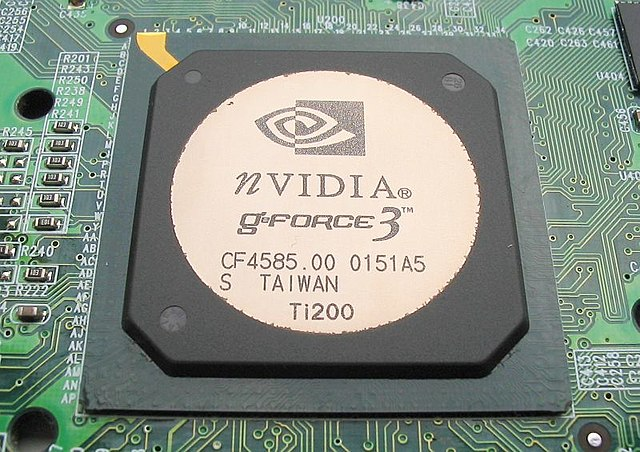
\includegraphics[width=8cm, height=5cm]{Imagens/GPU1.jpg}
\caption{GPU nVidia GeForce 3}
\end{figure} 

\section{Historia das GPUs}
\label{sect.Historia das GPUs}
Desde o inicio do uso de computadores pessoais as placas de vídeo eram necessárias, sendo que no começo todo o processo era garantido pela \ac{CPU}. Não existiam imagens em 3 dimensões, e possuíam pouca coloração, as imagens eram criadas pela \ac{CPU} e a Placa de Vídeo apenas repassavam os dados da imagem e passava-os para o frame, estas placas dependiam 100\% do restante sistema e comunicavam com a placa-mãe através da \textbf{interfarce ISA}, projetada para a época rodando em paralelo com clocks e tendo uma taxa de transferência muito baixa. 	

Com o surgimento das imagens \textbf{2D} as placas já utilizavam \textbf{interface PCI}, tendo clock e taxa de transferência mais altos. Continham circuitos mais completos e complexos para processar as imagens passaram a depender menos do \ac{CPU}, sendo possível utilizar uma interface gráfica mais sofisticada com design das janelas, renderização de textos sendo possível também a decodificação de imagens e vídeo em alguns formatos.

Com a vinda das imagens \textbf{3D} com mais complexidade e com a necessidade de uma \ac{GPU} mais capacitada surgiu a \textbf{interface AGP}, esta tinha uma taxa de transferência mais elevada do que os antigos \textbf{PCI} já ultrapassados. Esta interface tinha varias versões e por bastante tempo foram exclusivas para placas de video.

como já vínhamos num ciclo novamente com a evolução da qualidade das imagens, dos jogos e softwares, a \textbf{interface AGP} já estava ultrapassada, a solução foi eliminar barramentos paralelos, e introduzir uma conexão \textit{“point to point”} com clocks e tavas de transferência muito altas, surgem assim os \textbf{PCI Express}. Atualmente estamos na versão 4.0 desta interface, que tornou-se rapidamente o padrão na industria.

Por volta dos anos 2000, as placas-mãe começaram a conter os chamados \textit{“GPU onboard”} que apesar de suportarem aplicações \textbf{3D} não tinham capacidade para rodar jogos e aplicações pesadas. Apos alguns anos surgem no mercado as \ac{APU} criados pela AMD, estes chips eram uma \ac{CPU} com uma \ac{GPU} intefarre o que trazia bom desempenho, mas não dispensava o uso de placa de vídeo para obter maior desempenho e qualidade.

Atualmente os processadores Core da Intel trazem um adaptador gráfico, mas devido ao seu desempenho baixo, são apenas utilizado sem apoio da placa gráfica quando o computador apenas desempenha funções de escritório, sendo que para utilizar softwares mais pesados e poder rodar jogos é necessário o usa de uma placa de vido conectada ao slot \textbf{PCI Express}.  

\section{Desempenho}
\label{sect.Desempelnho}
O desempenho da \ac{GPU} depende de Vários fatores.

 
\begin{figure}
\center
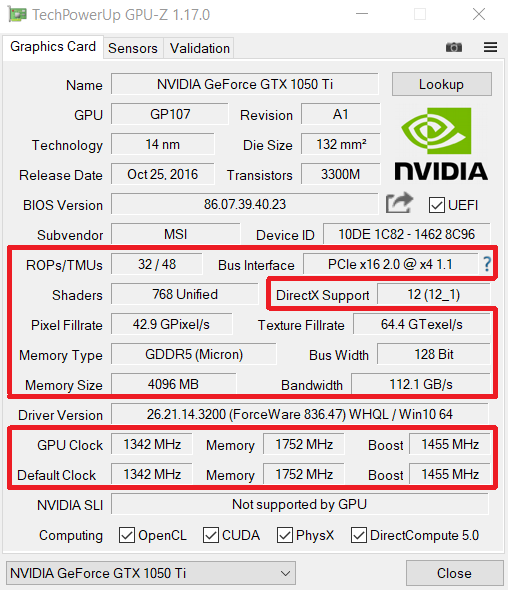
\includegraphics[width=8cm, height=8cm]{Imagens/desempenho.png}
\caption{1050 Ti em detalhes no App GPU-Z.}
\end{figure} 

\begin{itemize}
    \item ROPs/TMUs
    \item Shaders
    \item Pixel Fillrate
    \item Texture Fillrate
    \item Bus Interface
    \item Bus width
    \item Memory Type
    \item Memory Size
    \item Bandwidth
    \item GPU Clock
    \item Default Clock    
\end{itemize}

Com base nesta informação vamos explicar detalhadamente os termos destacados.

\subsection{Clock}
\label{sect.Clock}
\textbf{Clock} é um chip que vai definir o ritmo de processamento e a sincronização entre circuitos, as placas de vídeo possuem um cristal clock que cria um \textbf{frequência em Mhz}. Este sinal é enviado para o chip através de um circuito chamado \ac{PLL}, é gerado um sinal com algus Mhz e é utilizado para gerar a frequência para cada parte do circuito, sendo que cada uma trabalha em um ritmo diferente. As \textbf{GPUs} atuais possuem sistemas de gerenciamento de energia, sendo normal estarem a trabalhar a uma frequência inferior a sua capacidade, estas também tem um modo Boost que aumenta a frequência do clock (Overclock) utilizado por exemplo quando a demanda de processamento é elevada em jogos.

\subsection{Shaders}
\label{sect.Shaders}

São códigos que foram incluídos no final dos anos 90 para geram efeitos diversos nas imagens em jogos. As placas anteriores á implementação desta tecnologia não tem capacidade para rodar jogos, estes shaders são processados em circuitos específicos, existem vários tipos de shader.

\textbf{Vertex Shader} Utilizado em jogos e aplicações quando á a necessidade de mover polígonos e mudar a forma de objetos, aplicar detalhes, coisas que não seriam bem feitas utilizando apenas texturas ou seriam demasiado complexas para serem trabalhadas individualmente.

\textbf{Pixel Shader} Utilizado na etapa de renderização de imagens sendo utilizado na criação real de cenários através de uma Setup Engine, repleto de polígonos é enviado para uma fragmentação que server para distribuir o quando ao ser processado. Em jogos são utilizados na estrutura de objetos, sombras, efeitos de luz, cores, entre outros.

\textbf{Geometry Shader} Outro tipo de conjunto de instruções de shader, direcionado á criação de grupos de vértices, processados pelas shader units, permitindo ao desenvolvedor criar um cenário com muitos objetos sem sobrecarregar a \ac{CPU}.

\subsection{TMU}
\label{sect.TMU}

Sigla para \textit{“Texture Mapping Unit”} em português \textit{"Unidade de Processamento de Texturas”} trabalham conjuntamente com as Shader Units sendo responsáveis por aplicar textura nas imagens, sendo bastante mais simples que os Shader Units, podem ficar limitadas quando ativados filtros de textura. Isto pode agravar-se caso a comunicação com a memoria tenha baixa taxa de transferência.

\subsection{ROP}
\label{sect.ROP}

ROP \textit{“Raster Operation Units”} em português \textit{“Unidade de Operação Raster”}, apos uma imagem ser processada era fica arquivada em unidades ROPs que aplicam outros filtros á imagem. Os circuitos mais antigos eram constituídos pela mesma quantidade de \textbf{TMUs e ROPs} enquanto os atuais contem quantidades diferentes para obter um balanço na distribuição de recursos internos.  

\subsection{Controlador de memoria RAM}
\label{sect.Controlador de memoria RAM}

O controlo de memoria RAM serve para fazer a gestão das informações enviadas e recebidas através da RAM. Dentro deste á circuitos que enviam comandos de leitura, escrita, acesso a dados, etc.

\subsection{Interface}
\label{sect.Interface}

Como já vimos existem vários tipos de interfaces, e a taxa de transferência é um fator diretamente ligado á capacidade de processamento, permitindo que a transferência de dados seja feita em maior frequência.  

\chapter{CPU (Central Processing Unit)}
\label{chap.CPU}

Central Process Unit (\ac{CPU}), ou em português Central de Processamento, é a componente chave de qualquer computador, a \ac{CPU} é responsável por realizar e calcular as tarefas solicitadas pelo usuário. 

\begin{figure}
\center
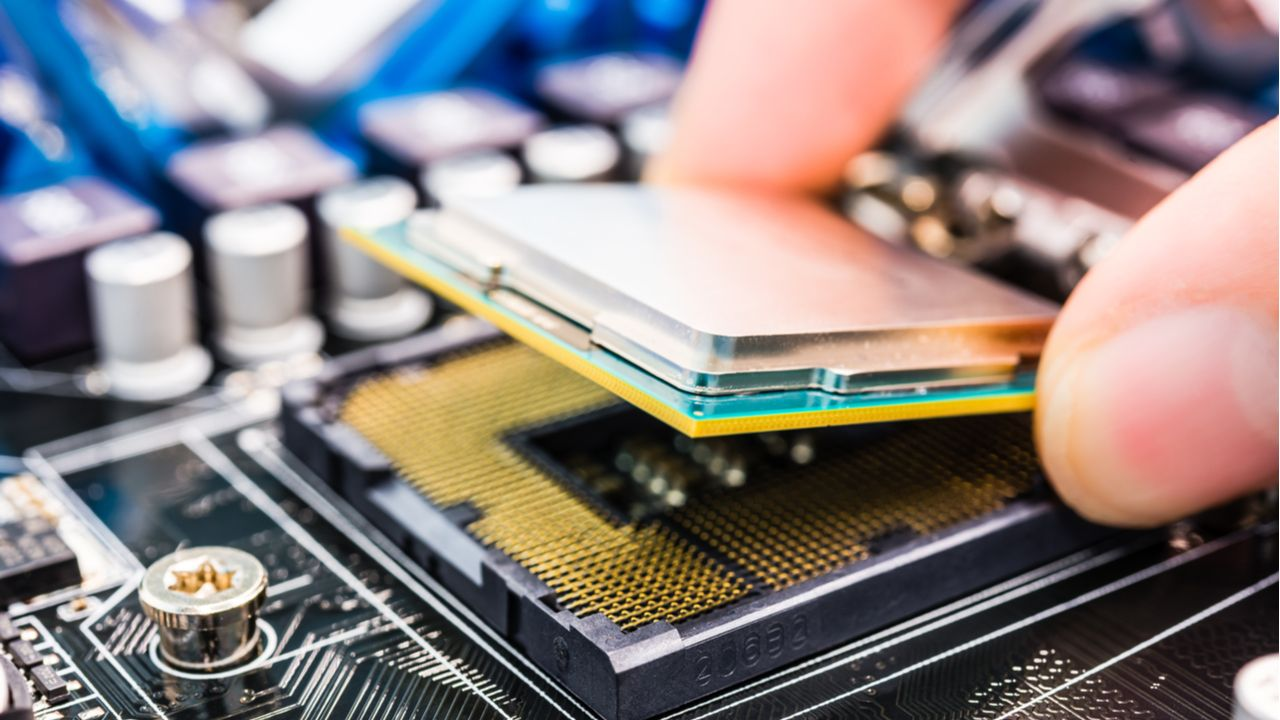
\includegraphics[width=4cm, height=4cm]{Imagens/cpu1.jpg}
\caption{A CPU é a componente mais importante do Computador}
\end{figure} 

A característica da \ac{CPU} tem influência direta no desempenho dos programas que estão a ser rodados no computador.

\section{História dos Processadores}
\label{sect.História dos Processadores}

Levamos décadas até chegar aos modelos utilizados atualmente, antes não era possível utilizar todos os softwares pois estes não eram compatíveis com todos os Hardwares, isto levou a cada computador utilizasse plataformas diferentes, e com isto chegava a haver incompatibilidade entre componentes do mesmo fabricante.

Os computadores primordiais eram bastante diferentes dos que conhecemos atualmente, comparados com os atuais estes n teriam capacidade de armazenar programas, chegando a haver projetos com a ideia de armazenar softwares no seu interior, mas esta ideia acabou por ser posta de lado.

Em 1945, surgiu a ideia de criar uma unidade capaz de executar diversas tarefas, esta ideia publicada por \textit{Jhon Von Neumann} foi a responsável pela origem dos primeiros modelos de processadores da forma que conhecemos atualmente. Durante a década de 50 começa a ser repensada a organização interna dos computadores, e os processadores começam a ter funcionalidades básicas.

No começo da década de 60, foi desenvolvida uma abordagem diferente, a \textbf{IBM} planejou uma família de computadores que poderia executar o mesmo Software, mas com diferente capacidade de processamento, passando os programas a deixarem de ser dependentes das máquinas.

\subsection{Geração Pré-x86}
\label{sect.Geração Pré-x86}

O \textbf{Intel 4004} foi o primeiro a ser lançado, desenvolvido para ser utilizado em calculadoras, este \ac{CPU} opera com um clock máximo de 740 KHz e tinha capacidade de calcular até 92 mil instruções por segundo a uma velocidade de 11ms.

\begin{figure}
\center
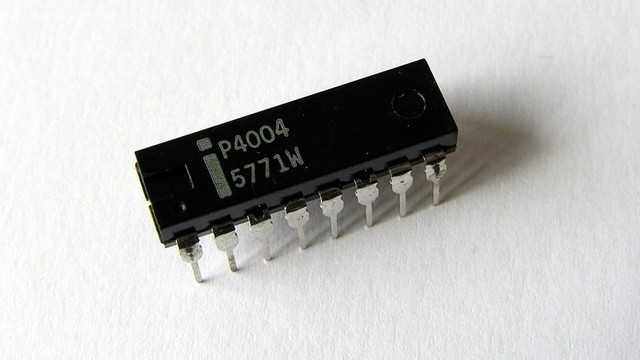
\includegraphics[width=4cm, height=4cm]{Imagens/intel4004.jpg}
\caption{Intel 4004}
\end{figure} 

Após o sucesso do \textbf{4004}, surge o \textbf{8008} em 1971 este era uma \ac{CPU} de 8 bits e tinha capacidade de armazenar o endereço de 16KB de memoria o seu clock trabalhava a uma frequência máxima de 0.8 Mhz.
Em 1974, este foi substituído pelo \textbf{intel 8080} que sendo 8 bits, podia executar algumas operações de 16 bits, este foi desenvolvido inicialmente para o controlo de misseis teleguiados, e podia fazer referência a cerca de 64kb de memoria.

\subsection{Processadores de 32 bits}
\label{sect.Processadores de 32 bits}

Com lançamento no final dos anos 80, estas trabalhavam com clocks que alcançavam valores até 100 Mhz, o \textbf{intel 80386} por exemplo já permitia que programas utilizassem o processador de forma cooperativa.

\begin{figure}
\center
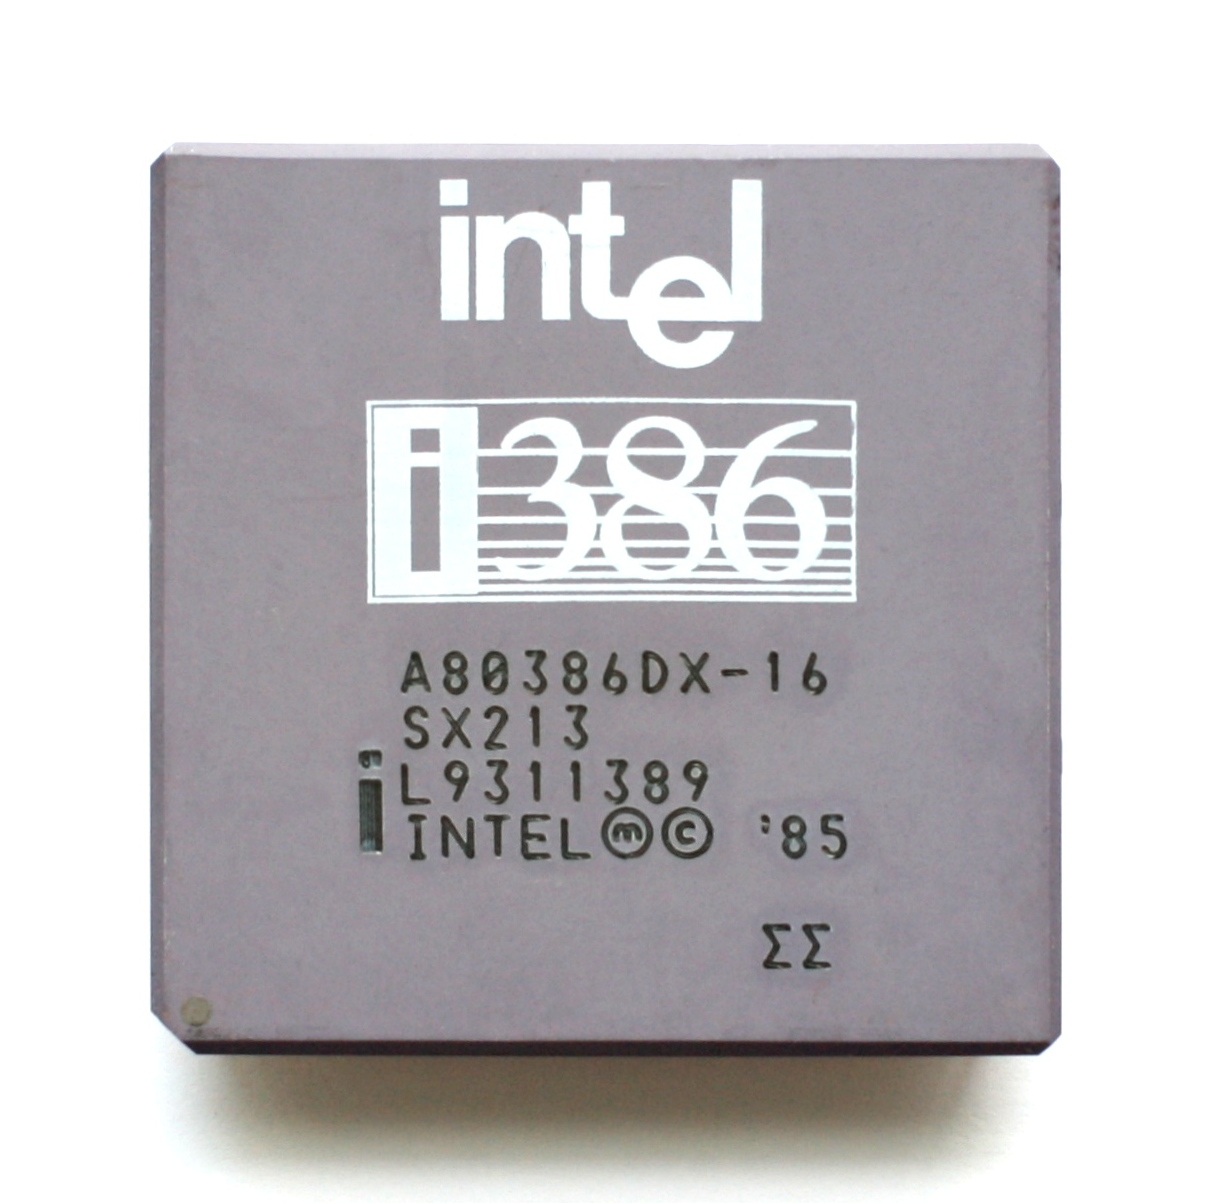
\includegraphics[width=4cm, height=4cm]{Imagens/intel80386.jpg}
\caption{Intel 80386}
\end{figure} 

\subsection{A luta entre Intel e AMD}
\label{sect.A luta entre Intel e AMD}

Após o lançamento do primeiro Pentium em 1993 que apresentava melhorias significativas em relação aos antigos modelos, com um clock inicial de 100 Mhz com o tempo acabou por chegar a 200 Mhz, em 1995 a intel lançou o Pentium Pro, a sexta geração dos x86.

Paralelamente a AMD começava a ganhar mercado com modelos semelhantes, o \textbf{AMD K5} concorrente ao primeiro Pentium mas poucos anos depois surgiu o \textbf{Pentium II} com clock capaz de atingir 450 Mhz, nessa mesma época aparecia os \textbf{AMD k6} com capacidade similar aos intel, por este motivo as empresas iniciaram uma corrida para quem alcançava o melhor desempenho.

\subsection{A lei de Moore}
\label{sect.A lei de Moore}

\begin{figure}
\center
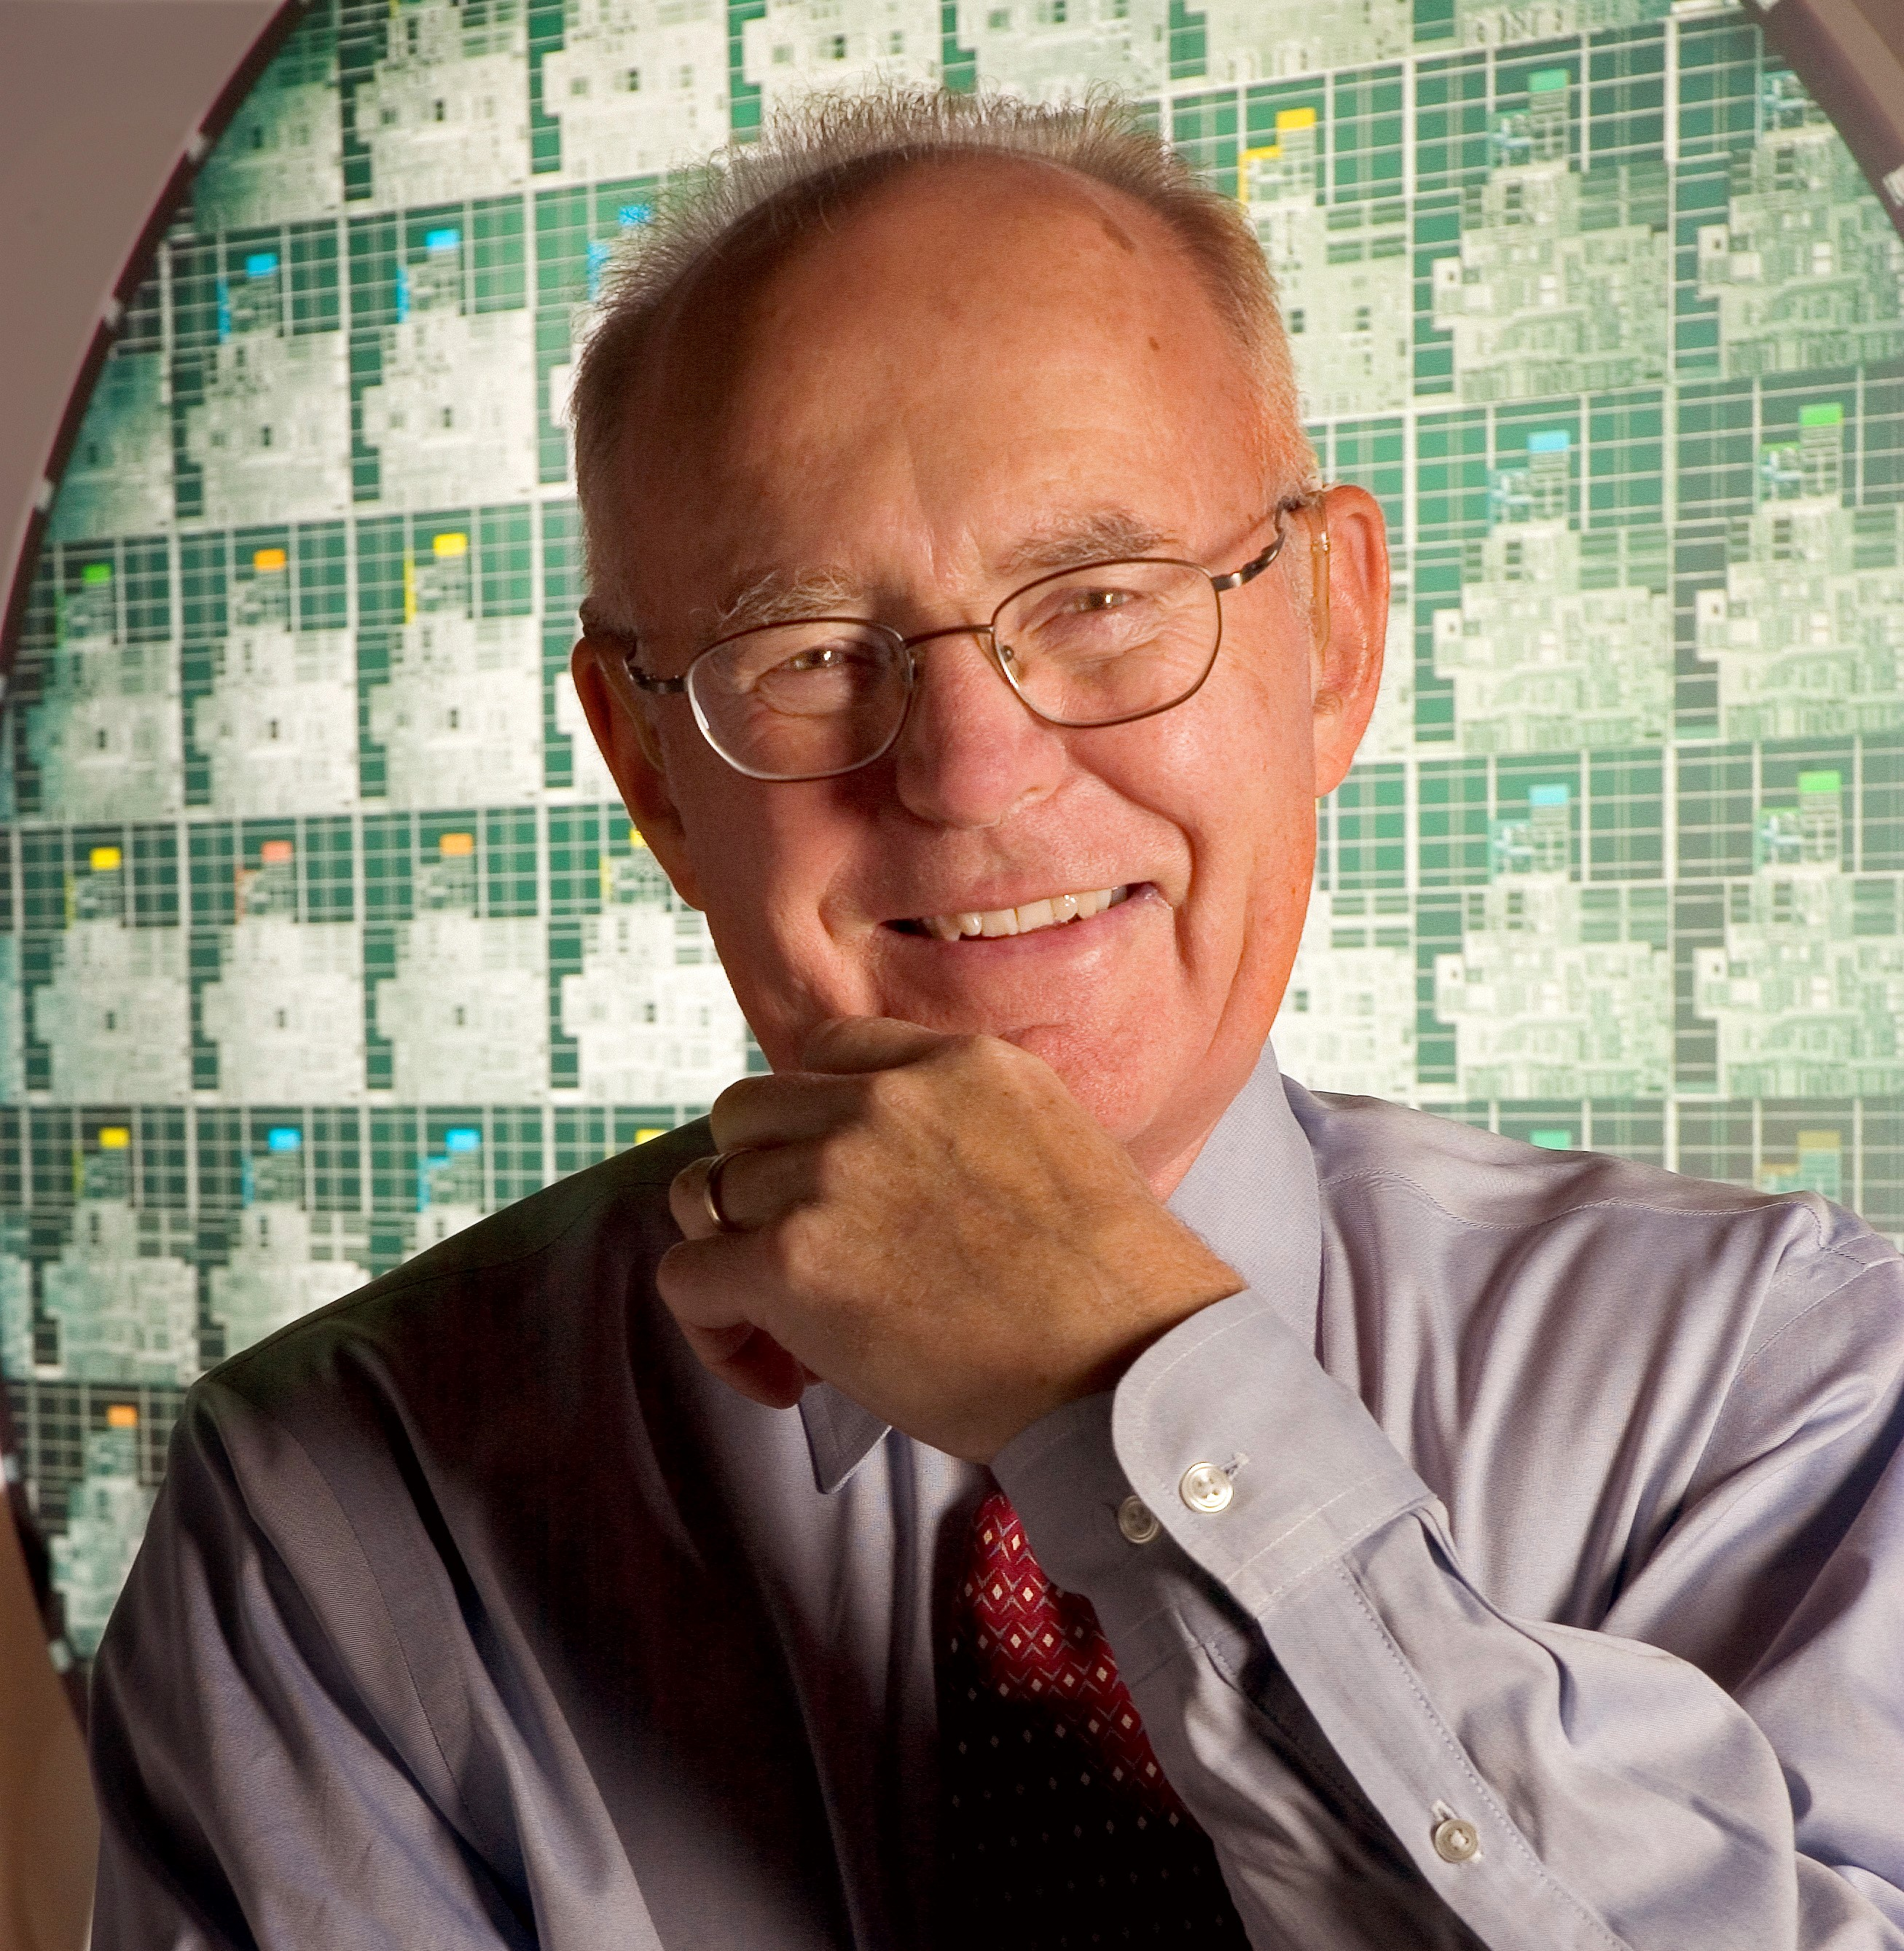
\includegraphics[width=6cm, height=6cm]{Imagens/gordonmoore.jpg}
\caption{Gordon Moore, Cofounder And Chairman Emeritus, Intel}
\end{figure} 


\textit{Gordon Moore} em 1965 afirmou que o numero de transístores em um chip dobraria a cada 18 meses sem custo adicional, \textbf{Lei de Moore}, que foi válida durante anos. Sempre que era lançado um novo modelo, meses de pois a concorrente acabaria por superar, isto foi bastante evidente no final dos anos 90
Mas a reviravolta vem quando a Intel lança o Pentium 4 em 2002, estre trabalhava com até 2GHz e meteu a empresa no topo do mercado.

\subsection{Multicore}
\label{sect.Multicore}

Conforme a evolução da tecnologia, o tamanho dos transístores foi diminuindo, no lançamento do \textbf{Pentium 4} estes já tinham 0.13 micrómetros e capacidade muito elevada, sendo fisicamente impossível aumentar o clock. A Soluçao a este problema foi começar a trabalhar com mais do que um núcleo em simultâneo, assim os núcleos passavam a trabalhar a uma frequência mais baixa, por exemplo um Dual-core de 1.3 Ghz passava a ter desempenho de um núcleo de 2.6 Ghz, um escalonador era utlizado para definir qual núcleo desempenhava a tarefa. 

Sendo assim a Lei de Moore tornou-se invalida, visto que já n era possível aumentar a frequência como antes.

\subsection{Era 64 bits}
\label{sect.Era 64 bits}

No começo da década de 2000, ficou evidente que o uso de 32 bit não poderia ficar mais eficiente sendo que no máximo apenas 4 GB de Memoria RAM poderiam ser endereçados com esta plataforma, sendo assim começou o desenvolvimento de arquiteturas a trabalhar em 64 bits.

Nesta altura as empresas entraram em acordo e licenciaram o uso dos x86-64 e x86-32 partilhando este hardware de forma legal, todos os modelos com processador de 64 bits rodam sobre o sistema x86-64

\subsection{Blackfin}
\label{sect.Blackfin}

Continuamos em 2000, surfe uma nova arquitetura de processadores, lançada pela \textbf{Analog Devices}, a Blackfin é uma família de microprocessadores de 16 e 32 bits, e trazia um DPS (processador de sinal digital) embutido para o processamento de áudio e vídeo.
Este processador permite um consumo menor de energia.

\subsection{Intel Core}
\label{sect.Intel Core}

Em 2006 a Intel iniciou a sua linha core para consumidores, desta linha faz parte \textbf{Core 2 Duo} que tinha uma capacidade elevada comparado aos antigos dual-core, na mesma época foi lançado o \textbf{Pentium Dual Core}, uma versão premium dos antigos, apesar de ser boa opção no custo beneficio era inferior ao \textbf{Core 2 Duo}, outro grande lançamento foi o \textbf{Core 2 Quad} que tinha um desempenho alto, mas os quatro núcleos acabavam por perder em algumas tarefas para os Dual Cor, mas mesmo assim eram capazes de chegar até 3.2 Ghz.

Em 2010 surgem os \textbf{Cores I}, sendo estes o \textit{i3 o i5 e o i7}, alguém disto a Intel lançou também muitas melhorias na arquitetura. 

\chapter{Degradação da Performance do Hardware}
\label{chap.Degradação}

	Com o aumento da populariedade de crypto-moedas e crypto-mining, surgiu uma ideia que leva consumidores a não desejarem comprar hardware (especialmente processadores e placas gráficas) que tenha sido préviamente utilizado para minerar crypto-moedas ou até outras tarefas como gaming e trabalhos profissionais como rendering, pois muitos acreditam que estas tarefas estam diretamente relacionadas à degradação da performance de \ac{CPU}s e \ac{GPU}s. Esta ideia levou à pergunta: Será que existe mesmo degradação da performance do hardware dos computadores?
	
	Para responder a esta questão, devemos primeiro dividir os componentes de computadores em diferentes categorias:
\renewcommand{\theenumi}{\Roman{enumi}}
\large{\begin{enumerate}
	\item Partes mecânicas, ou seja, partes que se movem fisicamente com outras partes.
	\item Componentes que têm reações químicas ao longo do tempo.
	\item Todos os outros componentes que não se encontram nas categorias anteriores, que neste caso serão maior parte dos componentes num computador.
\end{enumerate}}

\section{Partes Mecânicas}
\label{sect.Partes Mecânicas}
	Partes mecânicas têm necessidade de um movimento relativo entre as duas superfícies de contato, que devido à existencia de fricção, levam ao desgaste de ambas as superfícies. Isto é, quer seja um componente de um computador ou outro sistema qualquer, partes mecânicas irão sempre tender a a desgastar-se quanto mais forem utilizadas, ou seja, podemos concluir que irá existir perda de performance em partes mecânicas do Hardware de um computador e eventualmente estas irão falhar com o tempo. Exemplos deste tipo de Hardware são ventoinhas com a representada na \textbf{\autoref{fig.ventoinha}} (usadas para manter a temperatura do hardware dentro da sua temperatura de utilização), discos rígidos ou até mesmo periféricos como teclados, ratos e outros botões fisicos. 
\begin{figure}[h]
\center
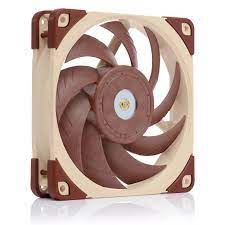
\includegraphics[width=5cm, height=5cm]{Imagens/fan1.jpg}
\caption{Ventoinha}
\label{fig.ventoinha}
\end{figure} 
	
\section{Componentes que Degradam por Reações Químicas e Magnéticas}
\label{sect.Reações Químicas}
	Degradação por reações químicas acontece em componentes como baterias que vão perdendo capacidade a cada ciclo de carga e descarga, alguns tipos de capacitores também se degradam por outras reações quimicas e, por exemplo, no caso dos discos rijidos (armazenamento por reações magnéticas) que também se encontram na categoria anterior, o computador irá mostrar sinais de lentidão ao longo do tempo pois os tempos de leitura e escrita destes irá degradar quanto mais estes sejam usados, embora para estes já haja alternativas como \ac{SSD}s que são  mais rápidos e estão menos sujeitos a degradação. Por outro lado, os discos rígidos ainda são os com maior capacidade de armazenamento.
	
\section{Resto dos Componentes}
\label{sect.Resto dos Componentes}	
	Apesar de haver muitos outros componentes, vamos testar apenas alguns dos principais componentes de processamento dos computadores, ou seja, \ac{CPU}s e \ac{GPU}s.
	
\subsection{Metodologia}
\label{subsect.Metodologia}
	Para testar se realmente existe degradação na performance deste tipo de hardware, será efetuada uma série de \textbf{ benchmarks}\footnote{Benchmarking serve como ponto de referência para a comparação de produtos} de várias tarefas (tanto video-jogos como programas de rendering e stress-testing\footnote{Processo para determinar a abilidade de um computador manter um certo nível de performance por um longo período de tempo}) de modo a podermos comparar a sua performance atual com o resultado da performance que o mesmo hardware teve à 2 anos atrás. O hardware que vai ser utilizado para esta experiência terá como \ac{CPU} um \textbf{AMD RYZEN 5 3600X} e o \ac{GPU} utilizado será um \textbf{AMD RADEON 5600XT}. Este hardware foi usado apenas para gaming durante o seu primeiro ano e está à pouco mais de um ano, ligado quase 24 horas por semana a fazer crypto-mining.
	Os jogos serão testados por uma função dentro do software oficial da \textbf{AMD(Radeon Software)} que permetirá ver a média de \ac{fps} que cada jogo obteve na duração do teste. Para obter resultados coerentes, cada jogo teve um tempo de medição de cerca de 10 minutos de modo estabilizar a temperatura e performance do hardware. Os jogos escolhidos foram \textbf{CS:GO, League of Legends, GTA V, Rainbow Six Siege, Assassin's Creed Origin, Shadow of the Tomb Raider, Final Fantasy XV e For Honor} pois eram os que já tinha feito o benchmark em 2019 quando montei o computador (ou seja, hardware estava completamente novo, o que dará mais credibilidade aos resultados), por isso não haverá nenhum título mais recente do que 2019. 
	De seguida, para um teste mais especifico para o \textbf{\ac{CPU}}, iremos usar progamas como o \textbf{Cinebench R 20, Cinebench R 15}, os quais são baseados no Cinema 4, que é um software utilizado mundialmente para rederizar e criar formas 3D. Também seram feitos benchmarks no \textbf{Geekbench 5} e no \textbf{Blender 2.81}(mais especificamente, um gráfico 3D popular para benchmarks com o nome "bmw27").
	Finalmente, para a testagem do \textbf{\ac{GPU}}, apenas serão feitos 2 benchmarks diferentes, \textbf{Furmark} (neste caso, esta benchmark era a única que não tinha feito em 2019, então fui ao site oficial da Furmark onde encontrei o resultado de um sistema similar ao meu) e \textbf{Heaven DX11 Benchmark}, sendo que este último irá fazer um stress-test ao \ac{GPU}.
	
\subsection{Resultados}
\label{subsect.Resultados}
\begin{center}
\textbf{\Large{Média de \ac{fps} em Jogos}\\\normalsize{(Definições de gráficos em ULTRA e Resolução 1080p)}}
\Large
\begin{tabular}{|c|c|c|}
	\hline
	\textbf{Jogo} & \textbf{2019} & \textbf{2021}\\ \hline
	CS:GO & 305.1 & 334.8\\	\hline
	League of Legends & 571.5 & 513.9\\	\hline
	GTA V & 88.5 & 93.0\\	\hline
	Rainbow Six Siege & 225.7 & 209.3\\	\hline
	Assassin's Creed Origin & 68.6 & 71.2\\	\hline
	Shadow of the Tomb Raider & 95.4 & 95.8\\	\hline
	Final Fantasy XV & 84.5 & 80.7\\	\hline
	For Honor & 152.1 & 185.3\\	\hline
\end{tabular}\\
\small(Maior é melhor)\\
\vspace{1cm}
\textbf{\Large{Pontuação do Ryzen 3600X (\ac{CPU})}}\\
\LARGE
\begin{tabular}{|c|c|c|}
	\hline
	\textbf{Programa} & \textbf{2019} & \textbf{2021}\\ \hline
	R 20 - Single-Core & 501 & 505\\	\hline
	R 20 - Multi-Core & 3751 & 3780\\	\hline
	R 15 - Single-Core & 204 & 217\\	\hline
	R 15 - Multi-Core & 1647 & 1709\\	\hline
	Geekbench 5 - Single-Core & 1245 & 1245\\ \hline
	Geekbench 5 - Multi-Core & 6992 & 7002\\ \hline
	Blender & 233.9s & 215.4s\\ \hline
\end{tabular}\\
\small (Maior é melhor, excepto no Blender que menor tempo é melhor)\\
\vspace{4cm}
\textbf{\Large{Pontuação do Radeon 5600XT (\ac{GPU})}}\\
\large
\begin{enumerate}
	\item Furmark\\
	Neste benchmark, o \ac{GPU} no sistema de composição similar ao meu, obteve uma pontuação de \textbf{5697} em 2019, enquanto no meu sistema foi obtida uma pontuação de \textbf{6507}.
	\item Heaven DX11 Benchmark
	
	\begin{figure}[h]
		\center
		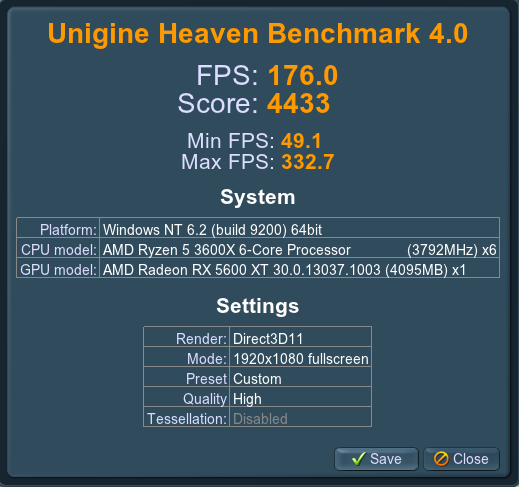
\includegraphics[width=6cm, height=6cm]{Imagens/HeavenDX11_0.png}
		\caption{Heaven Benchmark Results 2019}
		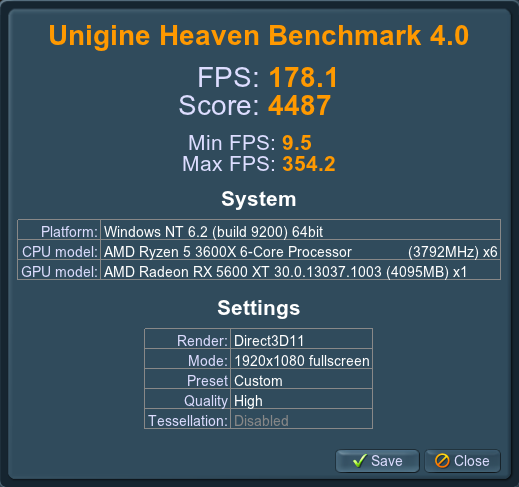
\includegraphics[width=6cm, height=6cm]{Imagens/HeavenDX11.png}
		\caption{Heaven Benchmark Results 2021}
		\label{fig.heaven}
	\end{figure}
\end{enumerate}
\end{center} 
\vspace{20cm}

\subsection{Análise dos Resultados}
\label{subsect.Análise}
	\begin{large}
		Refeltindo sobre os resultados obtidos anteriormente (\textbf{\autoref{subsect.Resultados}}) sobre a média de \ac{fps} que cada jogo teve, podemos observar que, em maior parte dos casos não há uma grande variação entre os valores apesar dos 2 anos de diferença. O caso onde houve maior variação foi no jogo \textbf{League of Legends} com a perda de cerca de 10\% da sua performance original.\\
		Os resultados obtidos posteriormente (avaliando a performance do CPU) mostram, pelo contrário ao que dizem os rumores da perda de performance com o tempo, que houve uma subida em todos os parâmetros testados (excepto na Geekbench 5 - Single-Core que se manteve igual) desde a data dos primeiros testes. Isto poderá ter acontecido devido a várias causas, as quais serão faladas com mais detalhe na sub\autoref{subsubsect.causas}.
		Por ultimo, ao examinar os resultados dos testes à \ac{GPU}, podemos observar que na segunda benchmark (\textbf{Heaven DX11 Benchmark}) também houve uma pontuação bastante parecida à pontuação original, no entanto, se analisarmos os resultados da primeira benchmark (\textbf{Furmark}), conseguimos perceber que houve uma diferença um pouco maior, de quase 15\% maior performance atualmente do que no original. Esta ultima diferença poderá ter justificação através da sub\autoref{subsubsect.causas}, mas o mais provável, como este foi o unico caso em que o hardware era diferente, é que a diferença seja dada devido a um fenómeno chamado de "silicone lottery". Este fenómeno será discutido na sub\autoref{subsubsect.lottery}.
	\end{large}
	
\subsubsection{O que poderá ter causado a diferença dos valores obtidos?}
\label{subsubsect.causas}
	Apesar de o hardware usado para efetuar os benchmarks tenha sido o mesmo, no período de 2 anos de diferença das datas dos testes, houveram alterações tanto nas aplicações e jogos, assim como houve atualizações do próprio sistema operativo ou até mesmo alterações nos próprios drivers\footnote{Um driver é essencialmente o software que trata da comunicação entre o sistema operativo (e as suas aplicações) e o hardware} do hardware.\\
	Contudo, ainda poderá existir outros motivos para a desigualdade dos resultados. Entre eles estará, por exemplo, a degradação da performance dos componentes responsáveis pelo arrefecimento do sistema (através da degradação das própria ventoinhas e/ou particulas como pó e outros que estejam a empedir o airflow desejado para o sistema) ou até por vezes, a degradação do disco rígido como referidos na \autoref{sect.Partes Mecânicas}.\\
	Todos estes fatores podem ter levado ás diferenças que obeservamos nos resultados, sendo que no geral, as atualizações dos drivers do hardware tendem a trazer melhorias para o desempenho do hardware, embora isto não seja sempre o caso. No entanto, com o tempo os requerimentos minimos de uso de software tende a aumentar pois os desenvolvedores de software tentam tirar vantagem dos avanços na evolução do hardware, fazendo desta forma parecer que a performance do hardware estará mesmo a degradar(o qual não é verdade como podemos confirmar com os resultados anteriores).
	
\subsubsection{O que é Silicone Lottery?\cite{siliclot}}
\label{subsubsect.lottery}
	Apesar de em papel, os chips de \ac{CPU}s e \ac{GPU}s de modelo igual terem as mesmas especificações, cada chip pode ter pequenas diferenças na sua capacidade de performance. Daí o termo "silicone lottery", ás vezes poderá-se "ganhar a loteria" e obter um chip que performe melhor que a média do mesmo modelo, no entanto também se pode perder, obtendo assim um chip com uma pior performance.
	
\chapter{Conclusão}
\label{chap.Conclusão}
	\begin{Large}
	\textbf{O que podemos concluir sobre a degradação da performance do hardware de computadors?}\\
	\end{Large}
	Segundo os resultados obtidos no \autoref{chap.Degradação}, podemos assim concluir que tanto \ac{CPU}s como \ac{GPU}s não perdem performance ao longo do tempo. Estes retêm a sua abilidade de processamento até ao dia em que deixarem de funcionar, no entanto haverá a possibilidade dos requerimentos minimos do software aumentar. \\
	
	\begin{Large}
		\textbf{O que podemos fazer para manter a performance do hardware estável?}\\
	\end{Large}
	Para preservar a performance do nosso hardware devemos manter o mesmo de forma poder operar dentro das temperaturas impostas pelo fabricante. Em relação às partes referidas na \autoref{sect.Partes Mecânicas} e na \autoref{sect.Reações Químicas}, estas deverão ser trocadas assim que a performance destas prejudique o funcionamento do resto do sistema.
	
	
\chapter*{Contribuições dos autores}
 A pesquisa sobre os conteúdos presentes nos \textbf{\autoref{chap.GPU} e \ref{chap.CPU}} foi feita por \textbf{\ac{LM}}. Os tópicos seguintes (\textbf{\autoref{chap.Degradação} e \ref{chap.Conclusão}}) foram resultado da pesquisa de \textbf{\ac{RP}}. O resto do trabalho e a formatação em \textbf{\LaTeX}  foi feita em conjunto por ambos os autores.\\
\begin{center}
	\Large{\textbf{Contribuição de cada autor:}}\\
	\begin{tabular}{|c|c|}
	\hline
	\ac{RP} & 45\%\\ \hline
	\ac{LM} & 55\%\\ \hline
	\end{tabular}\\
	\vspace{1cm}
	\begin{large}
		Code UA: infor2021-ap-g29
	\end{large}
\end{center}

%%%%%%%%%%%%%%%%%%%%%%%%%%%%%%%%%
\chapter*{Acrónimos}
\begin{acronym}
\acro{ua}[UA]{Universidade de Aveiro}
\acro{GPU}[GPU]{Graphics Processing Unit}
\acro{CPU}[CPU]{Central Process Unit}
\acro{PLL}[PLL]{Phase Locked Loop}
\acro{APU}[APU]{Accelerated Processor Unit}
\acro{RP}[RP]{Rúben Pequeno}
\acro{LM}[LM]{Luís Moura}
\acro{fps}[fps]{Frames Per Second}
\acro{SSD}[SSD]{Solid State Drive}
\end{acronym}

%%%%%%%%%%%%%%%%%%%%%%%%%%%%%%%%%
\printbibliography
\end{document}